\documentclass[12pt,letterpaper]{article}
\usepackage[utf8]{inputenc}
\usepackage{float, xcolor}

%----- Configuración del estilo del documento------%
\usepackage{graphicx, fancyhdr, lastpage}
\usepackage{enumitem, pifont}
\usepackage[left=2cm,right=2cm,top=1.8cm,bottom=2.3cm]{geometry}

\pagestyle{fancy}
\fancyhf{}
\rfoot{\textit{Página \thepage \hspace{1pt} de \pageref{LastPage}}}

%------ Paquetes matemáticos básicos --------%
\usepackage{amsmath, amssymb, amsthm}

\newcommand{\imp}{\rightarrow}
\newcommand{\vp}{\varphi}

\begin{document}

%------ Encabezado -------- %
\begin{center}
  \begin{minipage}{3cm}
    \begin{center}
      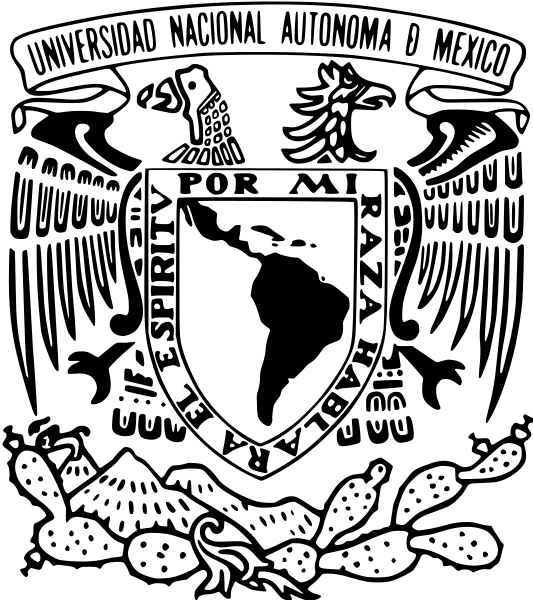
\includegraphics[height=3.4cm]{../unam_logo.png}
    \end{center}
  \end{minipage}\hfill
  \begin{minipage}{10cm}
    \begin{center}
      \textbf{\Large Universidad Nacional Autónoma de México}\\[0.2cm]
      \textbf{\large Facultad de Ciencias}\\[0.2cm]
      \textbf{Lógica Computacional | 2025-2}\\[0.4cm]
      \textbf{\Large Tarea 03}\\[0.1cm]
      \textbf{Docentes:}\\
      Noé Hernández \hspace{1em} Santiago Escamilla \hspace{1em} Ricardo López\\[0.3cm]
      \textbf{Autores:}\\
      Fernanda Ramírez Juárez \quad Ianluck Rojo Peña\\[0.3cm]
      \textbf{Fecha de entrega:} Martes 18 de marzo de 2025
    \end{center}
  \end{minipage}\hfill
  \begin{minipage}{3cm}
    \begin{center}
      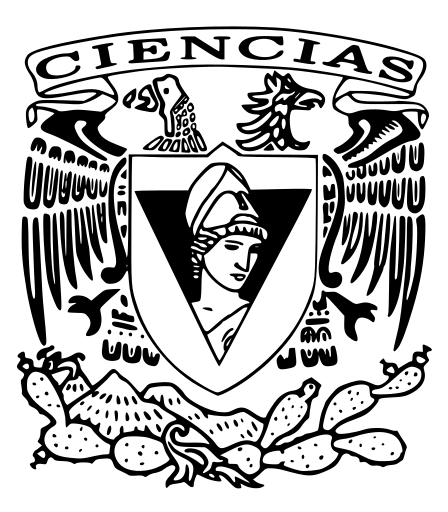
\includegraphics[height=3.4cm]{../fc_logo.png}
    \end{center}
  \end{minipage}
\end{center}

\bigskip
\hrule height 0.1pt
\bigskip

%------ Notas sobre la resolución --------%
\section*{Notas sobre la resolución.}

\begin{quote}
  \textbf{Nota general:}
  
\end{quote}

\bigskip
\hrule height 0.1pt
\bigskip

%------ Contenido -------- %
\section*{Resolución de Ejercicios.}

\begin{enumerate}

\item (1.5 pts.) Realice la especificación formal funcional acerca del tipo abstracto de datos pila, donde todos sus elementos son del tipo $A$. Utilice el predicado $P(x) : x$ es una pila de elementos de $A$, la constante para pila vacía \textit{empty}, y las funciones \textit{push}, \textit{pop} y \textit{top}, con su significado usual para pilas.
  \begin{enumerate}
  \item[a)] Definición del tipo de datos pila:
    \begin{enumerate}
    \item[\footnotesize I.] \textit{empty} es una pila vacía de elementos de $A$.
    \item[\footnotesize II.] El resultado de agregar un elemento de $A$ en el tope de la pila es una pila de elementos de $A$.
    \item[\footnotesize III.] Son todos.
    \end{enumerate}
  \item[b)] Si una pila no es vacía, entonces el elemento en el tope es un elemento de $A$.
  \item[c)] Si una pila no es vacía, entonces la pila que resulta de eliminar el elemento en el tope es una pila de elementos de $A$.
  \end{enumerate}
  \bigskip
  % -- Respuesta --
  \bigskip
  
\item (2 pts.) ¿Qué se sigue lógicamente de lo siguiente? \textit{Todos los monquitos son pachones. Pac es un monquito. Todos los chicubus son monquitos. Algunos monquitos son chicubus. Pac no es chicubus.}
  
  \vspace{0.2cm}
  
  \begin{center}
    \begin{tabular}{ll}
      a) Pac no es pachon. & d) Todos los chicubus son pachones. \\
      b) Todos los monquitos son chicubus. & e) Existen chicubus que no son pachones. \\
      c) Existen chicubus que no son monquitos. &
    \end{tabular}
  \end{center}
  
  \vspace{0.2cm}
  
  Traduzca el argumento, con la conclusión que haya seleccionado, a un secuente de la lógica de predicados, y halle una prueba de dicho secuente usando deducción natural. Use los predicados $M(x) : x$ es monquito, $P(x) : x$ es pachón, $C(x) : x$ es chicubus, y la constante $a$ para denotar a Pac.
  \bigskip
  % -- Respuesta --
  \bigskip
  
\item (2 pts.) Mediante deducción natural muestre la validez de:
  \begin{enumerate}
  \item[a)] $\exists x \exists y(S(x,y) \lor S(y,x)) \vdash \exists x \exists y S(x,y)$,
  \item[b)] $\forall x(P(x) \lor Q(x)), \exists x \neg Q(x), \forall x(R(x) \to \neg P(x)) \vdash \exists x \neg R(x)$.
  \end{enumerate}
  \bigskip
  % -- Respuesta --
  \bigskip
    
\item (1 pt.) Una fórmula atómica cerrada es una fórmula atómica $P(a_1, \dots, a_n)$ cuyos argumentos son constantes. Considere un lenguaje con $n$ objetos constantes y una sola relación \textit{binaria} $R^{(2)}$.
  \begin{enumerate}
  \item[\footnotesize I)] ¿Cuántas fórmulas atómicas cerradas hay en este lenguaje?\\
    a) $n$ \hfill
    b) $n^2$ \hfill
    c) $2^n$ \hfill
    d) $2^{n^2}$ \hfill
    e) $2^{2^n}$

  \item[\footnotesize II)] ¿Cuántas asignaciones de verdad son posibles en este lenguaje, i.e., cuántas posibilidades hay de definir $R^{\mathcal{M}}$?\\
    a) $n$ \hfill
    b) $n^2$ \hfill
    c) $2^n$ \hfill
    d) $2^{n^2}$ \hfill
    e) $2^{2^n}$
  \end{enumerate}
  \bigskip
  % -- Respuesta --
  \bigskip
  
\item (1.5 pts.) Sea $\varphi$ el enunciado $\forall x \forall y \exists z (R(x,y) \to R(y,z))$, con $R^{(2)}$.
  \begin{enumerate}
  \item[a)] Sea $A \overset{\text{def}}{=} \{a,b,c,d\}$ y $R^{\mathcal{M}} \overset{\text{def}}{=} \{(b,c), (b,b), (b,a)\}$. ¿Es cierto que $\mathcal{M} \models \varphi$? Justifique su respuesta.
  \item[b)] Sea $A' \overset{\text{def}}{=} \{a,b,c\}$ y $R^{\mathcal{M}'} \overset{\text{def}}{=} \{(b,c), (a,b), (c,a)\}$. ¿Es cierto que $\mathcal{M}' \models \varphi$? Justifique su respuesta.
  \end{enumerate}
  \bigskip
  % -- Respuesta --
  \bigskip
  
\item (2 pts.) Determine si el siguiente conjunto es satisfacible:
  \[
  \Gamma = \{P(b), Q(b), R(b), \exists x(P(x) \land \neg(Q(x) \lor R(x))), \forall x(R(x) \to P(x))\}
  \]
  \bigskip
  % -- Respuesta --
  \bigskip
  
\end{enumerate}
\end{document}
